\section{Capacidad de cómputo como activo económico}
\label{sec:compute_activo_economico}

El desarrollo y despliegue de sistemas de inteligencia artificial requiere
infraestructura especializada, energía y redes, y la expansión reciente de esta
capacidad ha aumentado la relevancia económica del cómputo
\parencite{stanford_ai_index_2026,iea_energy_ai_2025}. Para el análisis financiero
conviene distinguir entre la GPU física, que es un bien de capital, y el servicio
temporal que genera. En este trabajo el subyacente es este segundo concepto:

\begin{equation}
    P_t=\text{precio de alquiler de capacidad de cómputo en el instante }t,
\end{equation}

expresado según la fuente en unidades monetarias por GPU-hora. Una GPU-hora es un
servicio perecedero: la capacidad no utilizada en una hora no puede almacenarse
para consumirla posteriormente. Esta propiedad limita la aplicación directa de
los argumentos clásicos de almacenamiento y \textit{cash-and-carry}
\parencite{bandi_su_2026}. Por ello, el TFM trata el precio de acceso a compute
como una exposición económica no almacenable y no presupone la existencia de un
mercado completo de derivados sobre GPU-hora, aunque este tipo de contratos haya
comenzado a recibir atención regulatoria y de mercado
\parencite{cftc_compute_derivatives_2026}.

\section{Mercado de alquiler de GPU}
\label{sec:mercado_alquiler_gpu}

El precio de una GPU no es homogéneo entre proveedores ni modalidades. En los
mercados de infraestructura \textit{cloud} coexisten contratación
\textit{on-demand}, capacidad \textit{spot} o interrumpible y compromisos de
utilización de mayor duración, con diferencias en precio, disponibilidad y
flexibilidad \parencite{aws_ec2_ondemand,aws_ec2_reserved,google_cloud_spot_vms,
google_cloud_cud}. La literatura sobre cloud muestra que estas condiciones
contractuales forman parte del problema económico de adquisición de capacidad
\parencite{lin_pan_liu_2022}.

En consecuencia, una referencia de precio debe interpretarse condicionada por,
al menos, el modelo de GPU, la región y la modalidad contractual. Esta
heterogeneidad determina el tratamiento empírico del capítulo: la serie Ornn H100
se utiliza como referencia principal para caracterización y calibración, mientras
que las series SMM H100 aportan evidencia complementaria del mercado chino. No se
interpreta la diferencia entre ambas fuentes como un \textit{spread} arbitrable.

\section{Ornn Compute Price Index}
\label{sec:ornn}

La fuente principal es el \textit{Ornn Compute Price Index} (OCPI), una familia de
índices por modelo de GPU expresados en USD por GPU-hora. Su metodología utiliza
alquileres ejecutados de capacidad \textit{on-demand}, excluyendo cotizaciones
indicativas, capacidad reservada y contratos de largo plazo
\parencite{ornn_methodology_2026}. Para cada modelo, el índice se construye como
una media winsorizada ponderada por número de GPU:

\begin{equation}
    I_{g,t}
    =
    \frac{\sum_{i\in\mathcal{M}_{g,t}}n_i\widetilde p_i}
         {\sum_{i\in\mathcal{M}_{g,t}}n_i},
    \label{eq:ornn_index}
\end{equation}

donde $\widetilde p_i$ es el precio ejecutado tras la winsorización. La estructura
general es pública, pero los proveedores permanecen anonimizados y el percentil
exacto de winsorización no se divulga, por lo que el investigador externo no puede
reconstruir cada valor histórico desde sus componentes
\parencite{ornn_methodology_2026}.

El estudio utiliza el \textit{daily reference print} de NVIDIA H100 SXM accesible
mediante la API de Ornn \parencite{ornn_api_2026,ornn_faq_2026}. La muestra
congelada contiene \textbf{92 observaciones diarias entre el 26 de mayo y el 25 de
agosto de 2026}, en USD por GPU-hora. Esta serie es la única referencia de mercado
empleada para caracterizar la dinámica física y calibrar el Log-OU principal. La
copia local se conserva para reproducibilidad porque la ventana histórica accesible
puede variar con el tiempo. La extracción H100 se realizó el 26 de agosto de 2026;
el panel multi-GPU se extrajo el 27 de agosto de 2026, según los metadatos conservados.

\section{SMM y el mercado chino de capacidad de cómputo}
\label{sec:smm_china}

Como referencia del mercado chino se utiliza información de Shanghai Metals
Market (SMM). En 2026 SMM amplió su cobertura al alquiler de capacidad GPU y
anunció dos familias de datos: un índice de precios y una serie de
\textit{listing prices}, publicadas oficialmente desde el 3 de julio de 2026
\parencite{smm_compute_launch_2026}. La primera combina información de mercado
para construir una referencia estandarizada; la segunda refleja precios públicos
de oferta y no se interpreta como equivalente a una transacción ejecutada.

Las referencias SMM incorporan explícitamente dimensiones contractuales:

\begin{equation}
    \mathcal{S}
    =
    \{
        \text{modelo},
        \text{VRAM},
        \text{tipo de instancia},
        \text{región},
        \text{modalidad contractual}
    \}.
    \label{eq:smm_specification}
\end{equation}

Para el análisis principal se selecciona
\textit{SMM-H100-80G-Multi-GPU Node-WR-Monthly Reserved}
(SMM-GPU-CC-019), correspondiente a un nodo H100-80G en la región occidental de
China con contratación mensual. Como contraste regional se utiliza la referencia
equivalente para el delta del río Yangtsé (SMM-GPU-CC-005), cuya especificación
de referencia contempla un servidor dedicado con $8\times$ NVIDIA H100-80G
\parencite{smm_compute_prices_2026,smm_h100_yrd_2026}.

Ornn y SMM no representan contratos fungibles: Ornn mide capacidad
\textit{on-demand} por GPU-hora, mientras que la referencia china principal es
mensual y regional. La conversión a una unidad horaria no elimina las diferencias
de duración, disponibilidad, localización o configuración. Por ello SMM se utiliza
sólo como evidencia descriptiva complementaria y no interviene en la calibración
del modelo principal.

\section{Selección del H100 como subyacente principal}
\label{sec:seleccion_h100}

El estudio se centra en NVIDIA H100 como caso cuantitativo. La elección combina
relevancia tecnológica y, sobre todo, observabilidad: H100 aparece tanto en el
benchmark global de Ornn como en las referencias regionales de SMM
\parencite{nvidia_h100_2026,ornn_markets_2026,smm_compute_prices_2026}. Mantener
constante la arquitectura reduce una fuente de heterogeneidad al comparar ambos
mercados, aunque no elimina las diferencias contractuales.

La serie H100 SXM de Ornn queda fijada \textit{ex ante} como subyacente principal.
Las referencias H200, B200, A100 SXM4 y RTX 5090 disponibles en Ornn se reservan
para contraste descriptivo y no se utilizan para seleccionar retrospectivamente
el modelo o recalibrar el experimento \parencite{ornn_markets_2026}.

\begin{figure}[htbp]
    \centering
    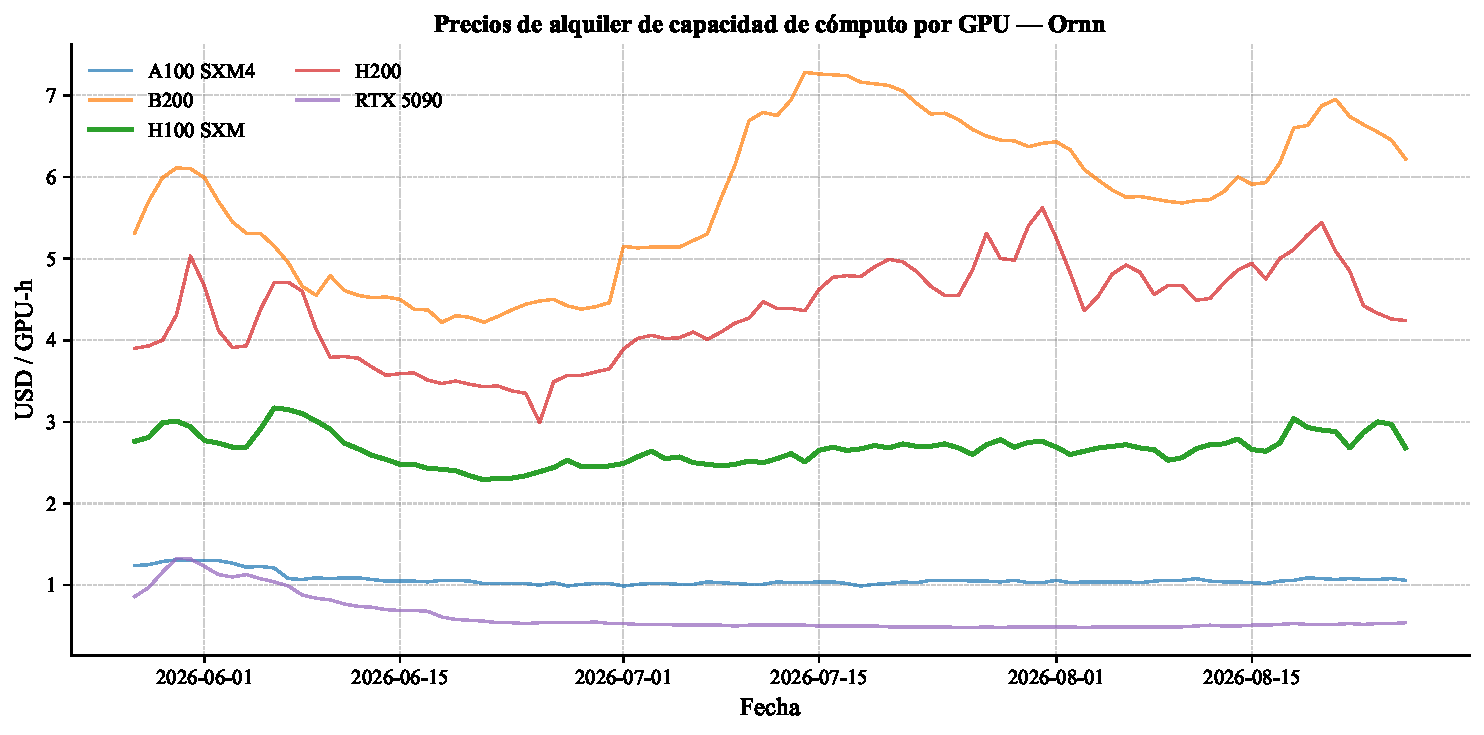
\includegraphics[width=0.92\textwidth]{../figures/market/01_ornn_gpu_price_levels.pdf}
    \caption{Evolución de los precios de alquiler por GPU en Ornn durante la muestra analizada. Panel extraído el 27/08/2026.}
    \label{fig:ornn_gpu_price_levels}
\end{figure}

La selección debe interpretarse como un estudio de caso y no como un índice
representativo de todo el mercado de compute. Otras generaciones de GPU pueden
presentar niveles, liquidez y dinámicas temporales diferentes y requerirían una
recalibración específica.

\section{Tratamiento de las series y construcción de variables}
\label{sec:tratamiento_datos}

Los datos originales se conservan sin modificación y las transformaciones se
realizan sobre copias derivadas. La muestra principal de Ornn queda congelada en
las 92 observaciones indicadas anteriormente. Para SMM se conserva igualmente una
extracción fija de las referencias Western Region y Yangtze River Delta. Dado que
la familia SMM fue lanzada después del inicio de algunas observaciones históricas
incluidas en la extracción, esos registros se interpretan como historia facilitada
por la fuente y no como evidencia de publicación en tiempo real anterior al
lanzamiento.

La limpieza convierte fechas y precios a tipos válidos, excluye registros sin
fecha o precio utilizable y ordena cronológicamente cada serie. En los diagnósticos
de una misma serie se conserva la última observación si una fecha aparece repetida.
La muestra principal Ornn H100 contiene 92 precios positivos, sin fechas duplicadas,
valores ausentes en fecha o precio ni huecos diarios entre sus extremos. Los campos
opcionales no utilizados pueden estar vacíos. No se aplica un recorte adicional de
valores extremos a los índices preservados: la winsorización de Ornn pertenece a
la construcción del índice por su proveedor. En SMM se mantienen las fechas
disponibles, sin interpolar ni rellenar días sin publicación; las comparaciones
utilizan únicamente fechas comunes. Al tratarse de índices de alquiler, no proceden
ajustes por dividendos o splits de acciones, y se conserva separada cada referencia
contractual.

Para estudiar cambios relativos se emplea el log-retorno

\begin{equation}
    r_t=\ln\left(\frac{P_t}{P_{t-1}}\right),
    \label{eq:log_return_data}
\end{equation}

mientras que para la calibración Log-OU se trabaja con el log-precio

\begin{equation}
    X_t=\ln P_t.
    \label{eq:log_price_data}
\end{equation}

Las comparaciones entre fuentes se restringen a fechas comunes,

\begin{equation}
    \mathcal{T}_{ij}=\mathcal{T}_i\cap\mathcal{T}_j,
    \label{eq:common_dates}
\end{equation}

y, para evitar interpretar diferencias de moneda, nivel y contrato como
diferencias directamente comparables, cada serie se normaliza a Base 100:

\begin{equation}
    B_t=100\,\frac{P_t}{P_{t_0}}.
    \label{eq:base100}
\end{equation}

Las correlaciones se utilizan únicamente como medidas descriptivas de
co-movimiento y no como evidencia causal o de integración de mercados:

\begin{equation}
    \rho_{ij}
    =
    \frac{\operatorname{Cov}(r_{i,t},r_{j,t})}{\sigma_i\sigma_j}.
    \label{eq:data_correlation}
\end{equation}

\section{Comparación descriptiva entre el mercado global y chino}
\label{sec:comparacion_global_china}

La Figura~\ref{fig:ornn_smm_base100} compara las referencias H100 global y chinas
tras normalizarlas a Base 100. El objetivo es estudiar su evolución relativa, no
construir un precio común ni un diferencial negociable.

\begin{figure}[htbp]
    \centering
    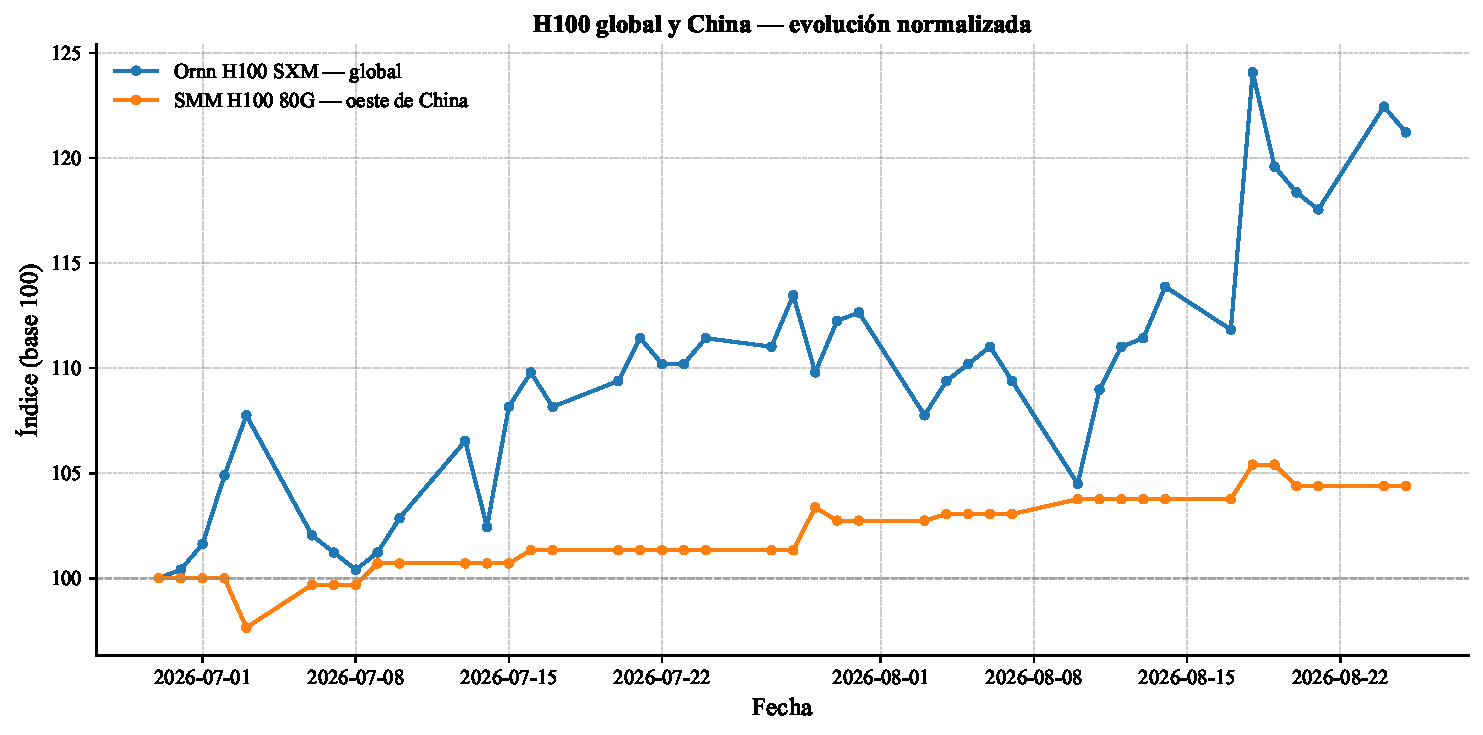
\includegraphics[width=0.90\textwidth]{../figures/market/02_h100_global_china_base100.pdf}
    \caption{Evolución normalizada del precio H100: Ornn y SMM. Muestras congeladas el 26/08/2026.}
    \label{fig:ornn_smm_base100}
\end{figure}

Durante la ventana disponible, Western Region aumenta aproximadamente un
$4{,}39\%$ y Yangtze River Delta un $9{,}63\%$. En las 42 fechas comunes de la
comparación principal, la correlación en niveles Base 100 es aproximadamente
$0{,}777$ para Ornn--Western Region y $0{,}704$ para Ornn--Yangtze River Delta:

\begin{equation}
\rho(B^{\mathrm{Ornn}},B^{\mathrm{West}})\approx0.777,
\label{eq:corr_base100_west}
\end{equation}

\begin{equation}
\rho(B^{\mathrm{Ornn}},B^{\mathrm{YRD}})\approx0.704.
\label{eq:corr_base100_yrd}
\end{equation}

Sin embargo, el co-movimiento desaparece al analizar variaciones de corto plazo:
la correlación de log-retornos es aproximadamente $-0{,}136$ con Western Region
y $0{,}036$ con Yangtze River Delta. Estos resultados aconsejan no interpretar
la elevada correlación de niveles normalizados como evidencia de integración de
mercados o de una relación de equilibrio.

\begin{equation}
\rho(r^{\mathrm{Ornn}},r^{\mathrm{West}})\approx-0{,}136,
\label{eq:corr_returns_west}
\end{equation}

\begin{equation}
\rho(r^{\mathrm{Ornn}},r^{\mathrm{YRD}})\approx 0.036.
\label{eq:corr_returns_yrd}
\end{equation}

\section{Limitaciones de los datos}
\label{sec:limitaciones_datos}

La principal limitación es la longitud de la muestra. Las 92 observaciones de
Ornn permiten una caracterización exploratoria y una especificación parsimoniosa,
pero no identifican con precisión propiedades estructurales de largo plazo. La
historia SMM es todavía más corta. Esta restricción motiva el uso posterior de un
Log-OU de un factor y el análisis de incertidumbre mediante bootstrap.

La segunda limitación es contractual. Ornn y SMM difieren en modalidad,
localización y construcción del benchmark; normalizar las series no elimina estas
diferencias. Por ello la comparación global--China es exclusivamente descriptiva.

La tercera es de transparencia. Ornn publica la metodología general del OCPI, pero
no la composición detallada de proveedores ni todos los parámetros necesarios para
reconstruir el índice. SMM, por su parte, combina distintas fuentes de información
de mercado. En ambos casos se conservan localmente las muestras utilizadas y los
benchmarks se tratan como observaciones externas.

Finalmente, H100 no representa todo el mercado de compute y las referencias
regionales seleccionadas tampoco representan todo el mercado chino. La
heterogeneidad observada entre arquitecturas y regiones impide extrapolar
automáticamente los resultados a otras GPU.

